\section{Grammar Definition}
\label{appendix:grammar}
Below, we provide the grammar definition used to generate verbal descriptions from the probability distribution over words estimated by the model.
Note, however, that no grammar was used during the learning phase: the speech recognizer used as a frontend to the spoken descriptions is based on a loop of words with no grammar, and the \AffWords{} model is based on a bag-of-words assumption, where only the presence or absence of each word in the description is considered.

%\begin{figure}
%  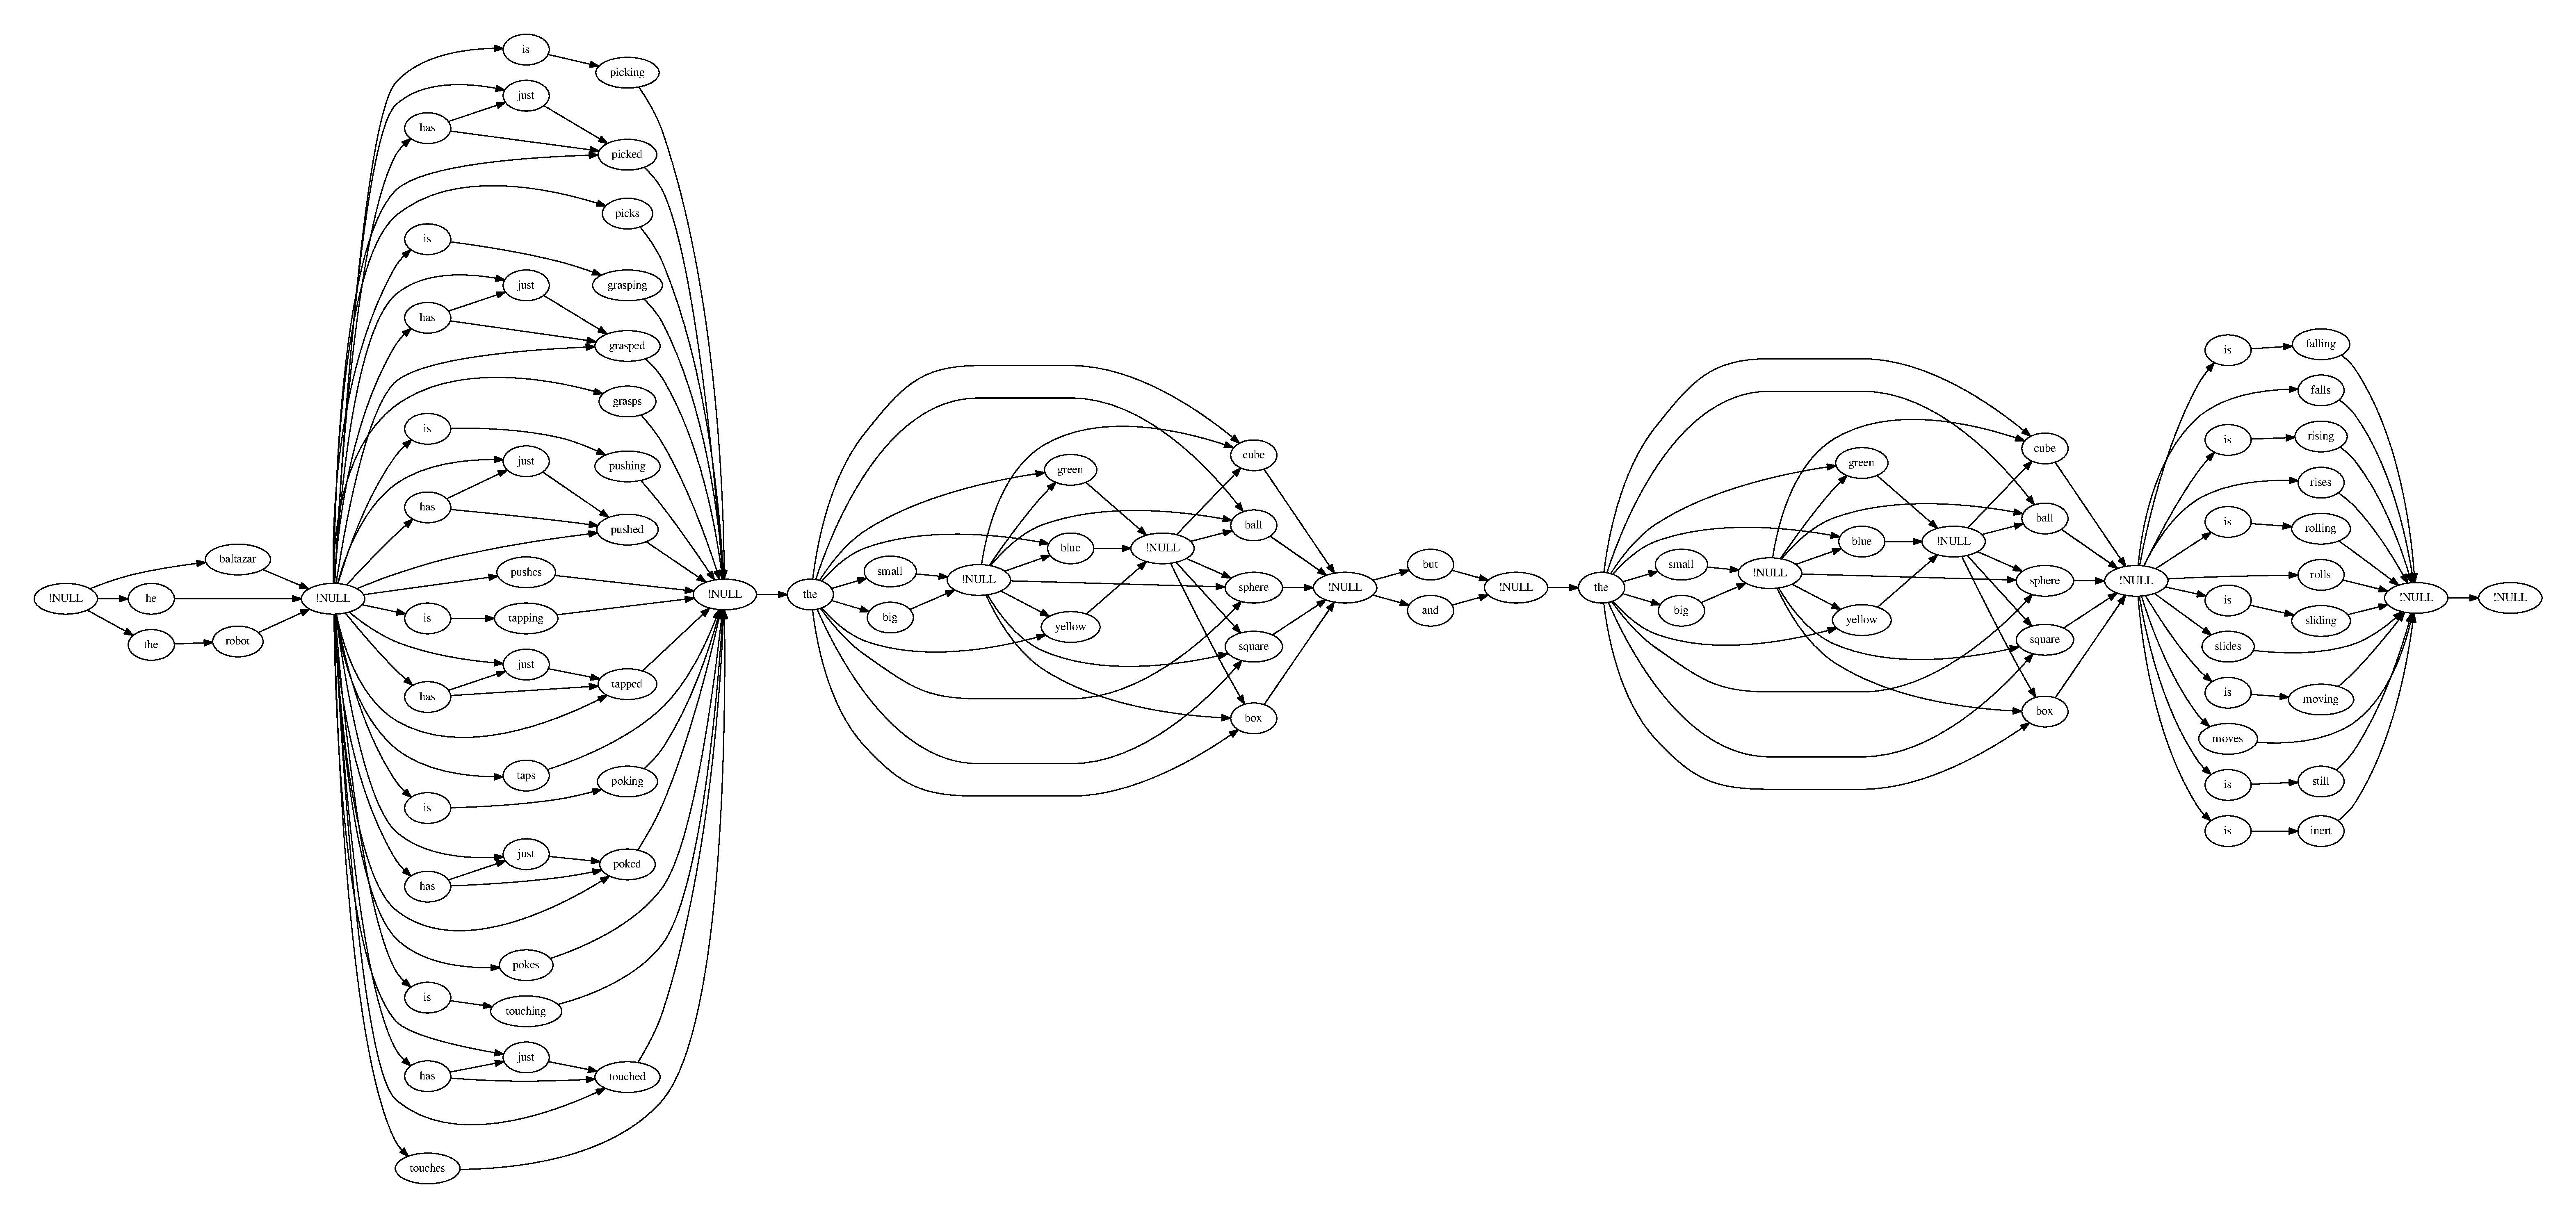
\includegraphics[width=\textwidth, angle=90]{figures/grammar}
%  \caption{Graphical representation of the formal \acf{CFG} used to generate descriptions from word probability distribution.}
%  \label{fig:grammar}
%\end{figure}

\begin{grammar}
  <sentence> ::= <agent> <action> <object> <conjunction> <object> <effect>

  <agent> ::= the robot | he | baltazar 

  <action> ::= <touch> | <poke> | <tap> | <push> | <grasp> | <pick>

  <touch> ::= touches | [has] [just] touched | is touching

  <poke> ::= pokes | [has] [just] poked | is poking

  <tap> ::= taps | [has] [just] tapped | is tapping

  <push> ::= pushes | [has] [just] pushed | is pushing

  <grasp> ::= grasps | [has] [just] grasped | is grasping

  <pick> ::= picks | [has] [just] picked | is picking

  <object> ::= the [<size>] [<color>] <shape>

  <size> ::= big | small
  
  <color> ::= green | yellow | blue
  
  <shape> ::= sphere | ball | cube | box | square

  <conjunction> ::= and | but

  <effect> ::= <inertmove> | <slideroll> | <fallrise>

  <inertmove> ::= is inert | is still | moves | is moving

  <slideroll> ::= slides | is sliding | rolls | is rolling

  <fallrise> ::= rises | is rising | falls | is falling
\end{grammar}

